\section{Paper 4}
\subsection{\emph{"A Data Set for Camera-Independent Color Constancy"}}

\begin{frame}{INTRODUCTION}
    In computer vision, the output generated by an algorithm depends on the 
    nature of the images set given as input. When the images come from 
    different sources (e.g. different cameras), the behavior of the algorithm is 
    not always the same. For this reason, we try to standardize the input in 
    order to have a more uniform output.
\end{frame}

\begin{frame}{COLOR CONSTANCY DATASETS}
    To produce uniform output, an algorithm must achieve "{\bfseries{color 
    constancy}}" on all input images. In order to calculate this property, there 
    are supervised and unsupervised algorithms. To test the performance of 
    these algorithms, there are already state-of-the-art datasets \footfullcite{0807099130} \footfullcite{0807099132} \footfullcite{0807099120}
    containing indoor and outdoor images, but these have few images inside 
    them.
\end{frame}

\begin{frame}{THE PROPOSED INTEL-TUT DATA SET}
    The purpose of the paper is to present a dataset containing images useful 
    for researching the {\bfseries{camera/scene-independence}} effect of an algorithm.
    To achive this, each scene was captured under five different illumination. 
    In each scene there are images taken from three different cameras, 
    including a mobile one.
    \begin{figure}[htbp]
        \centering
        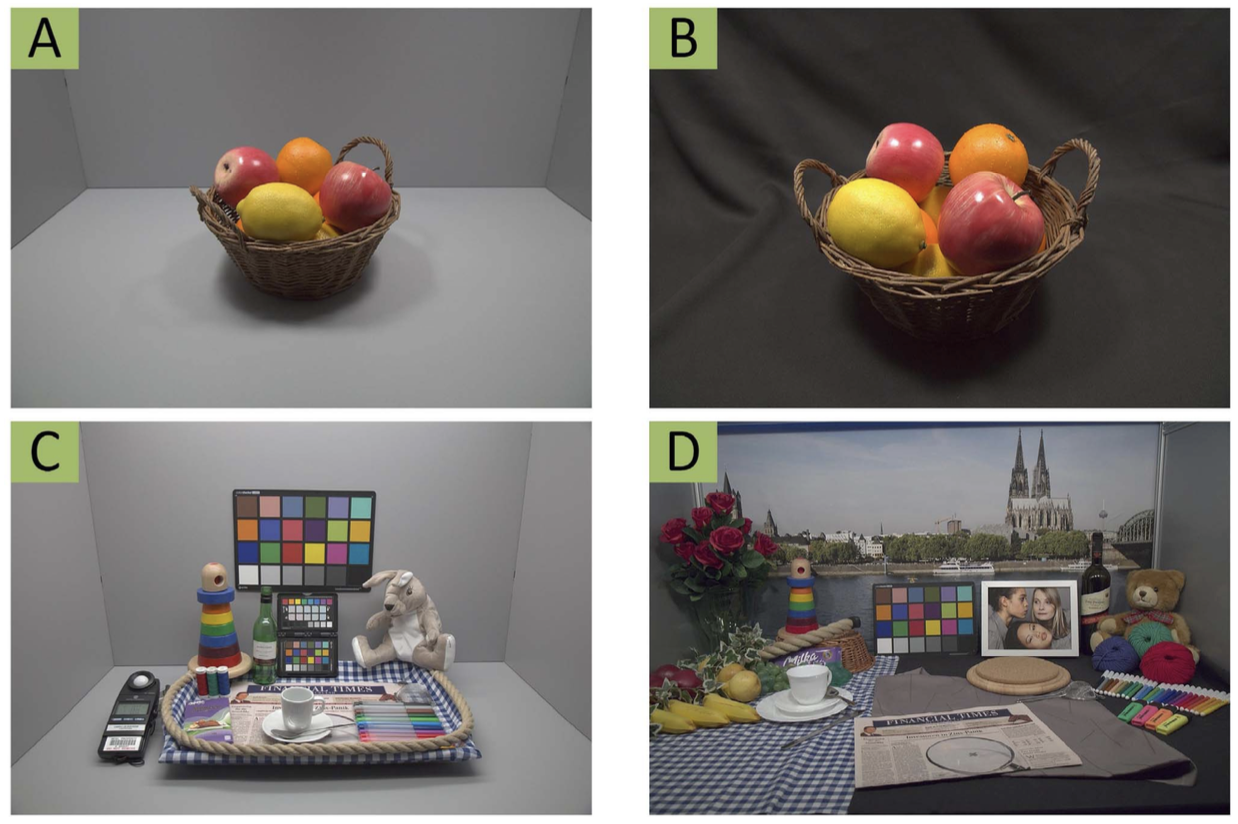
\includegraphics[width = 0.6 \linewidth]{images/paper4/lab.png}
        \centering
        \caption{Lab real scenes}
        \label{fig:Lab}
    \end{figure}
\end{frame}

\begin{frame}{THE PROPOSED INTEL-TUT DATA SET - Chromaticity}
    \begin{block}{Chromatic adaptation - \href{https://en.wikipedia.org/wiki/Color_vision}{\underline{Wikipedia}}}
        \emph{"In color vision, chromatic adaptation refers to color constancy; the 
        ability of the visual system to preserve the appearance of an object under 
        a wide range of light sources."}
    \end{block}
    The only information available on the light source are: the "\emph{Spectral 
    Power Distributions}" (SPD) and the "\emph{Spectral Reflectance}" (SR)
    Thanks to this information, we can obtain the existing chromaticity in the image 
    and compare it with that obtained from the "\emph{Camera Spectral Senstivities}" (CSS).
    \begin{block}{Target}
        The goal is to be able to bring the white point, calculated by each 
        algorithm, closer to the white point of the ground truth, within the same 
        color spectrum (sRGB). To do this, a "\emph{Color Conversion Matrix}" (CCM) 
        is used.
    \end{block}
\end{frame}

\begin{frame}{THE PROPOSED INTEL-TUT DATA SET - Evaluations}
    The performance of supervised and unsupervised methods can be 
    evaluated with 5 of the following strategies:
    \begin{enumerate}
        \item Camera Independence \label{CI}
        \item Camera and Scene Independence
        \item Camera and Scene Independence from Single Camera
        \item Testing the Effect of Color Shading
        \item Testing the Effect of Resolution
    \end{enumerate}
    In each of these strategies, the training set, validation set and testing 
    set contain, in different positions, different images acquired from different 
    cameras.
\end{frame}

\begin{frame}{EXPERIMENTAL RESULTS - Unsupervised methods}
    \begin{block}{Recover Angluar Error}
        Given the chromaticity estimated by the algorithm ($ p^{Est} $) and the 
        effective chromaticity (white point or ground truth) ($ p^E $), the 
        performance of an algorithm can be evaluated based on the result 
        returned by the "\emph{Recovery Angular Error}" (RAE):
        $$ RAE=\cos^{-1}\left(\frac{p^Ep^{Est}}{||p^E||~||p^{Est}||}\right) $$
    \end{block}
    \begin{figure}[htbp]
        \centering
        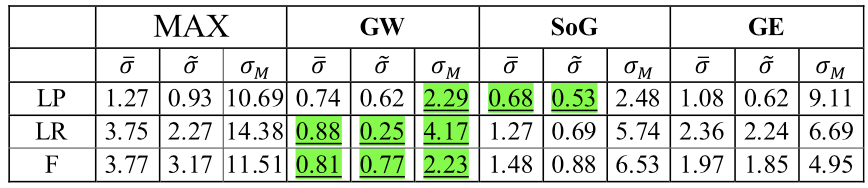
\includegraphics[width = 0.8 \linewidth]{images/paper4/standardHigh.png}
        \centering
        \caption{Mean, Median and Maximum RAE of some algorithms. GW \footfullcite{0807099104} achieves the best performance}
        \label{fig:RAEstandard}
    \end{figure}
\end{frame}

\begin{frame}{EXPERIMENTAL RESULTS - Supervised methods}
    Color constancy can also be calculated from convolutional neural networks (\emph{CCNs}) such as the one proposed in \footfullcite{0807099125}
    \begin{figure}[htbp]
        \centering
        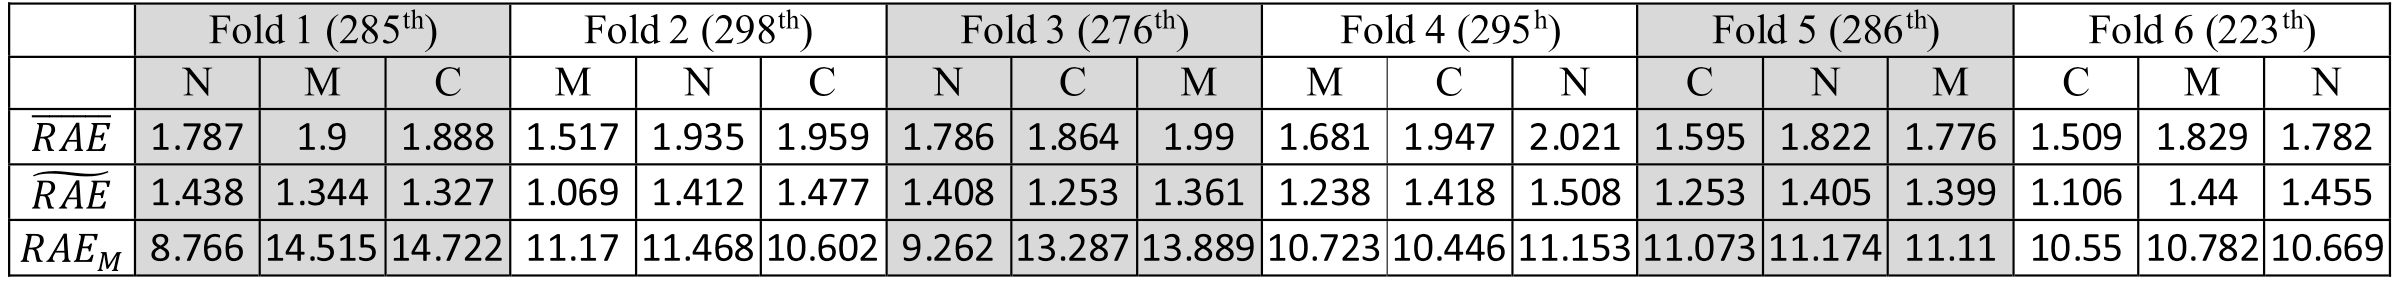
\includegraphics[width = 1 \linewidth]{images/paper4/25tech1.png}
        \centering
        \caption{Camera Independence with CCM on $ 1^{nd} $ thecnique. Mean, Median and Maximum RAE of CNN.}
        \label{fig:CNNtec1}
    \end{figure}
    \begin{minipage}{\linewidth}
        \centering
        \begin{minipage}{0.45\linewidth}
            \begin{figure}[H]
                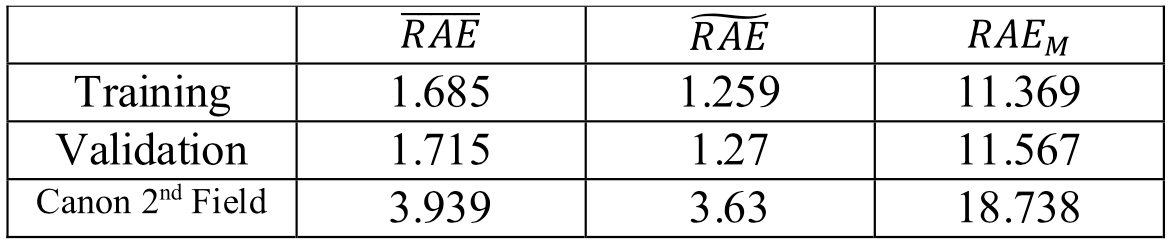
\includegraphics[width=\linewidth]{images/paper4/25tech2.png}
                \caption{\small Camera Independence on $ 2^{nd} $ thecnique. Mean, Median and Maximum RAE of CNN.}\label{fig:1}
            \end{figure}
        \end{minipage}
        \hspace{0.05\linewidth}
        \begin{minipage}{0.45\linewidth}
            \begin{figure}[htbp]
                \centering
                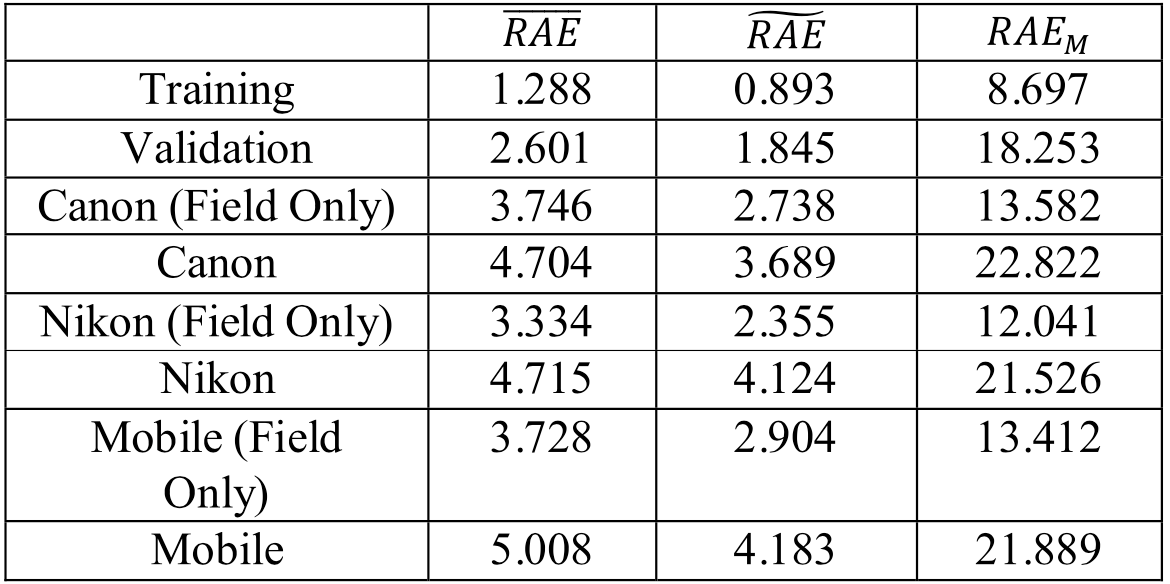
\includegraphics[width=0.8\linewidth]{images/paper4/25tech3.png}
                \caption{\small Camera Independence on $ 3^{nd} $ thecnique. Mean, Median and Maximum RAE of CNN.}\label{fig:1}
                \centering
            \end{figure}
        \end{minipage}
    \end{minipage}
\end{frame}
    
\begin{frame}{CONCLUSION}
    The dataset proposed in this paper is useful for testing the behavior of 
    an algorithm, or a model based on CNN, in the search of camera/scene-independece. 
    Achieving this goal can also be done using a CNN if the CMM process is 
    applied to its input set. It is necessary to specify that, in order to 
    achieve the final result, it is essential to have the spectral sensitivities of each camera 
    without which it would not be possible to achieve camera independence.
    \begin{figure}[htbp]
        \centering
        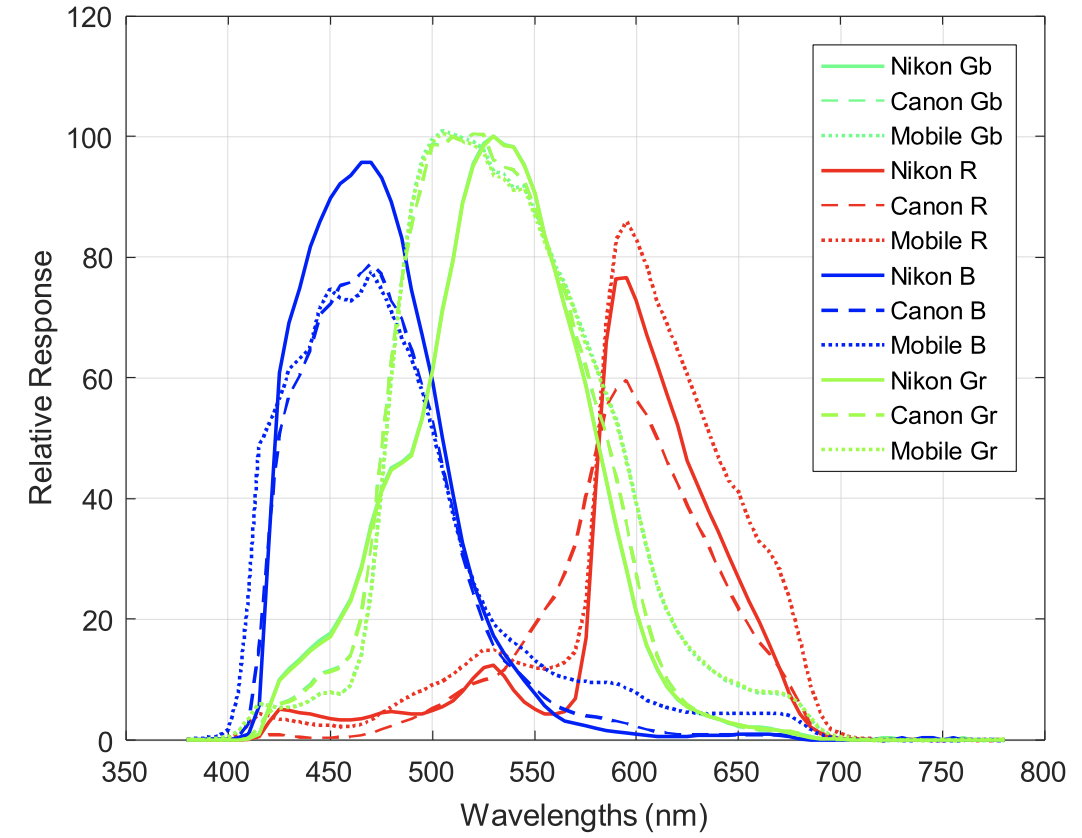
\includegraphics[width = 0.5 \linewidth]{images/paper4/CSS.png}
        \centering
        \caption{Camera Spectral Sensitivities (CSS) of the light sources.}
        \label{fig:CNNtec1}
    \end{figure}
\end{frame}